\documentclass{if-beamer}
% --------------------------------------------------- %
%                  Presentation info	              %
% --------------------------------------------------- %
\title[Advanced Bioinformatics]{Introduction to the Linux command line, NGS data formats, read mapping and alignments.}
\subtitle{Advanced Bioinformatics}
\author{Lecturer: Fernando Pozo} \
\institute[UFV]{
  \begin{normalsize}
  \href{mailto:fpozoc@cnio.es}{fpozoc@cnio.es}
  \end{normalsize}
\\~\\
  Bioinformatics Unit, \\
  Spanish National Cancer Research Centre (CNIO) 
}
\usepackage{datetime}
\newdate{date}{03}{09}{2019}
\date{\displaydate{date}}
\logo{

\includegraphics[scale=0.1]{logo.jpg}
}
\subject{Presentation subject} % metadata

\graphicspath{{figures/}}
% --------------------------------------------------- %
%                    Title + Schedule                 %
% --------------------------------------------------- %

\begin{document}

\begin{frame}
  \titlepage
\end{frame}

\begin{frame}{Schedule}
  \tableofcontents
\end{frame}

% --------------------------------------------------- %
%                      Presentation                   %
% --------------------------------------------------- %

\section{Next-generation sequencing (NGS)}
% --- %
% -1- %
% --- %
\begin{frame}{Why next-generation sequencing?}
\framesubtitle{\emph{Sanger vs. NGS}}
\begin{large}
\begin{itemize}
    \item For almost 30 years, sequencing of DNA has largely been dependent on the \nth{1} generation Sanger dideoxy sequencing method. 
    \item Sanger sequencing requires each sequence read to be amplified and read individually. Despite considerable improvements in automation and throughput, Sanger sequencing remains relatively expensive and labor intensive.
\end{itemize}
\exemple{In both technologies}:
\begin{itemize}
    \item DNA Polymerase adds fluorescent nucleotides one by one onto a growing DNA template strand. 
    \item Each incorporated nucleotide is identified by its fluorescent tag.
\end{itemize}
\end{large}
\end{frame}
% --- %
% -2- %
% --- %
\begin{frame}{Why next-generation sequencing?}
\framesubtitle{\emph{Sanger vs. NGS}}
\begin{large}
\begin{itemize}
    \item The critical difference between Sanger sequencing and NGS is \emph{sequencing volume}.
    \item While the Sanger method only sequences a single DNA fragment at a time, \emph{NGS is massively parallel, sequencing millions} of fragments simultaneously per run. 
    \item NGS high-throughput process translates into sequencing hundreds to thousands of genes at one time.
\end{itemize}
\end{large}
\end{frame}
% --- %
% -3- %
% --- %
\begin{frame}{Why next-generation sequencing?}
\framesubtitle{\emph{Sanger vs. NGS}}
\begin{huge}
“With Sanger sequencing, we saw a limited DNA snapshot… NGS and its massively parallel sequencing enable us to look at tens to hundreds of thousands of reads per sample.”
\end{huge}
\\~\\
Professor, Head of TrEnD laboratory, Curtin University
\end{frame}
% --- %
% -4- %
% --- %
\begin{frame}{Why next-generation sequencing?}
\framesubtitle{\emph{Sanger vs. NGS}}
\begin{figure}
\centering
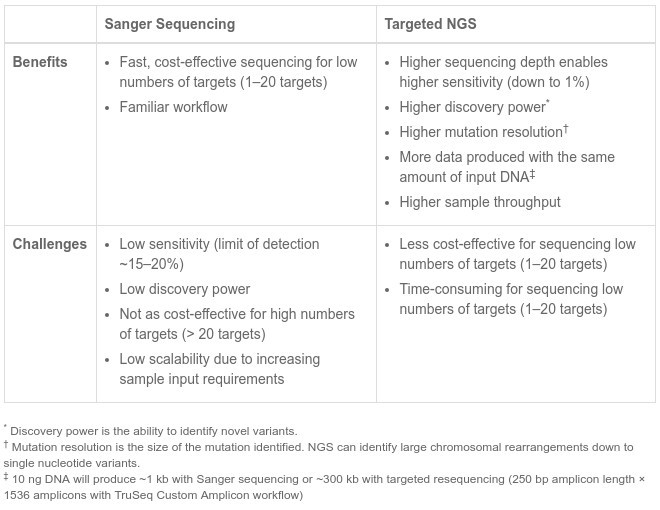
\includegraphics[scale=0.35]{sanger_sequencing.jpg}
\caption{Challenges and Benefits of Sanger Sequencing and NGS}
\end{figure}
\end{frame}
% --- %
% -5- %
% --- %
\begin{frame}{Why next-generation sequencing?}
\framesubtitle{\emph{Sanger vs. NGS}}
\begin{figure}
\centering
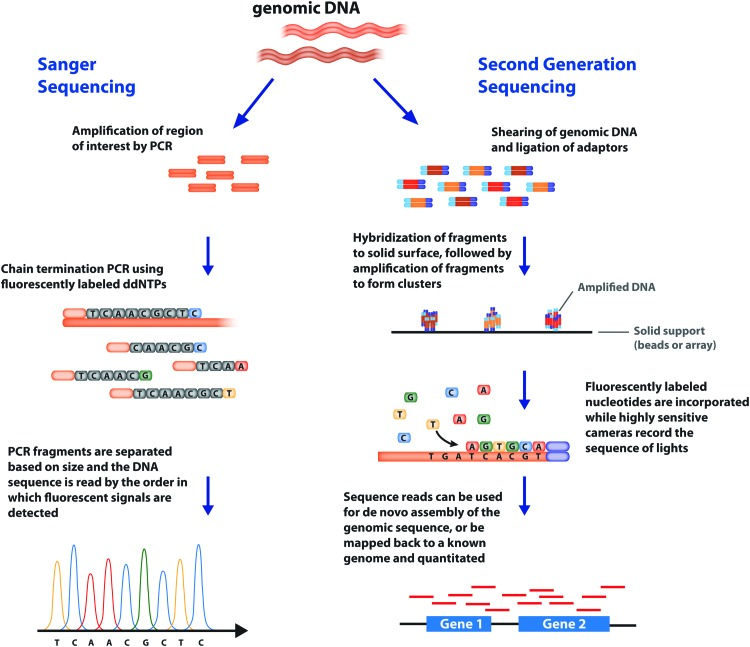
\includegraphics[scale=2.25]{comparison_sanger_ngs.jpg}
\caption{NGS platforms can sequence millions of DNA fragments in parallel in one reaction}
\end{figure}
\end{frame}
% --- %
% -6- %
% --- %
\begin{frame}{Why next-generation sequencing?}
\framesubtitle{\emph{Sanger vs. NGS}}
\begin{figure}
\centering
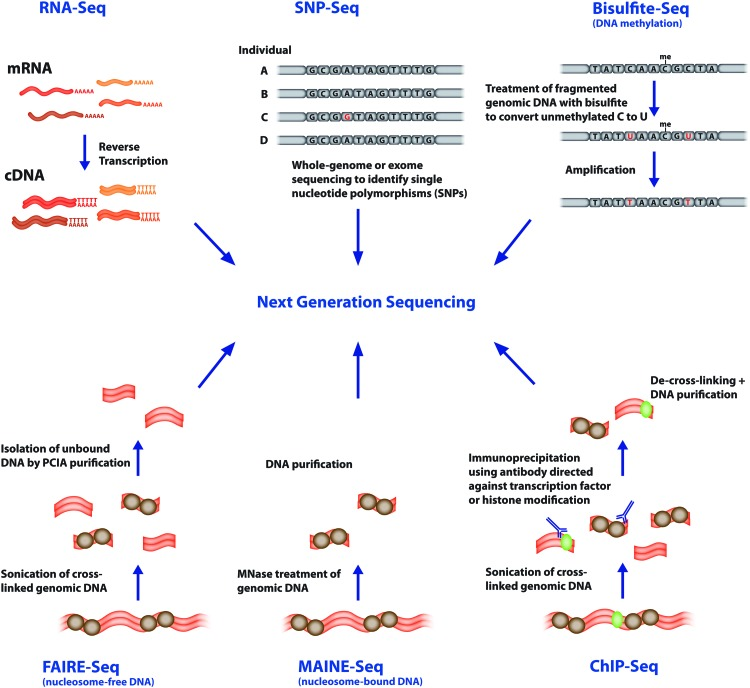
\includegraphics[scale=2.25]{applications_of_ngs.jpg}
\caption{The types of experiments that can be performed using NGS are many fold}
\end{figure}
\end{frame}
% --- %
% -7- %
% --- %
\begin{frame}{NGS platforms}
\begin{large}
\begin{itemize}
    \item \cref{https://www.ncbi.nlm.nih.gov/pubmed/16056220}{Roche 454 platform} (Roche Life Sciences).
    \item \cref{https://www.ncbi.nlm.nih.gov/pubmed/16081699}{Applied Biosystems SOLiD platform} (Applied Biosystems).
    \cref{http://www.cs.toronto.edu/~kriz/cifar.html}{CIFAR-10}
    \item \cref{https://www.ncbi.nlm.nih.gov/pubmed/18987734}{Illumina Genome Analyzer} (formerly known as Solexa) and HiSeq platforms (Illumina). 
    \item \cref{https://www.ncbi.nlm.nih.gov/pubmed/21776081/}{Ion Torrent} (Termofisher).
    \item 3rd generation sequencing (Single molecule level \& Longer Reads): 
    \begin{itemize}
        \item \cref{https://www.ncbi.nlm.nih.gov/pmc/articles/PMC4678779/}{PacBio Sequencing} (PacBio)
        \item \cref{https://genomebiology.biomedcentral.com/articles/10.1186/s13059-016-1103-0}{MinION} (Oxford Nanopore).
    \end{itemize}
\end{itemize}
\end{large}
\end{frame}
% --- %
% -8- %
% --- %
\begin{frame}{NGS protocol design}
\begin{exampleblock}{Quality Scores}
Measure the probability that a base is called incorrectly. It uses the phred-like algorithm (similar to that originally developed for Sanger).
\end{exampleblock}
% --- %
% -9- %
% --- %
\begin{exampleblock}{Paired-End vs. Single-End}
\begin{itemize}
  \item Paired-end sequencing allows users to sequence both ends of a fragment and generate high-quality, alignable sequence data. It facilitates detection of genomic rearrangements and repetitive sequence elements, as well as gene fusions and novel transcripts.
  \item Producing twice the number of reads for the same time and effort in library preparation, sequences aligned as read pairs enable more accurate read alignment and the ability to detect insertion-deletion (indel) variants, which is not possible with single-read data. All Illumina next-generation sequencing (NGS) systems are capable of paired-end sequencing.
\end{itemize}
\end{exampleblock}
\end{frame}
% --- %
% -10- %
% --- %
\begin{frame}{NGS protocol design}
\begin{exampleblock}{Multiplex Sequencing}
Processing more samples in less time. Sample multiplexing exponentially increases the number of samples sequenced per run
\end{exampleblock}
\begin{exampleblock}{Read Length}
Number of base pairs (bp) sequenced from a DNA fragment. The right sequencing read length depends on your sample type, application, and coverage requirements.
Examples: 
\begin{itemize}
  \item Long reads: \textit{de novo} assembly and resolving repetitive areas of the genome with greater confidence.
  \item Other applications: shorter reads are sufficient and more cost-effective than longer ones
\end{itemize}
\end{exampleblock}
\end{frame}
% --- %
% -11- %
% --- %
\begin{frame}{NGS protocol design}
\framesubtitle{\emph{Read Length for Different Applications}}
\begin{figure}
\centering
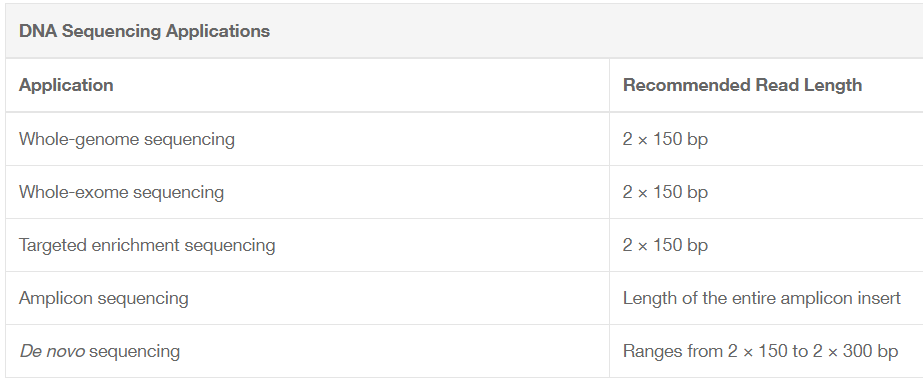
\includegraphics[scale=0.4]{dna_sequencing_applications.PNG}
\end{figure}
\end{frame}
% --- %
% -12- %
% --- %
\begin{frame}{NGS protocol design}
\framesubtitle{\emph{Read Length for Different Applications}}
\begin{figure}
\centering
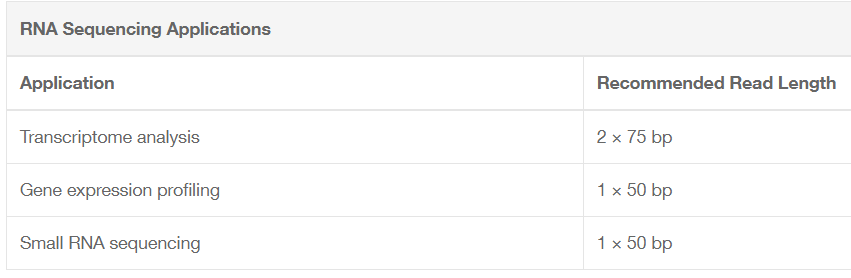
\includegraphics[scale=0.45]{rna_sequencing_applications.PNG}
\end{figure}
\end{frame}
% --- %
% -13- %
% --- %
\begin{frame}{NGS protocol design}
\begin{exampleblock}{Coverage}
Average number of reads that align to known reference bases. Variant discovery can be made with a certain degree of confidence at particular base positions.
\end{exampleblock}
\begin{figure}
\centering
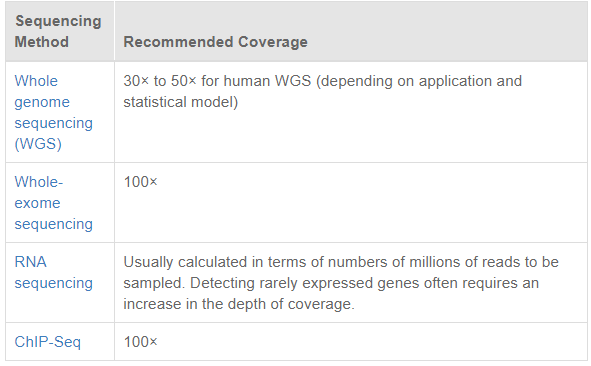
\includegraphics[scale=0.5]{sequencing_coverage_requirements.PNG}
\caption{Sequencing Coverage Requirements}
\end{figure}
\end{frame}
% --- %
% -14- %
% --- %
\begin{frame}{NGS protocol design}
\begin{exampleblock}{Deep Sequencing}
Sequencing a Genomic region multiple times, sometimes hundreds or even thousands of times.
\\~\\
The case of Cancer Research: Required sequencing depth increases for low purity tumors, highly polyclonal tumors, and applications that require high sensitivity (identifying low frequency clones). Cancer sequencing depth typically ranges from 80× to up to thousands-fold coverage.
\\~\\
Factors Impacting Cancer Sequencing Depth:
\begin{itemize}
    \item Purity of the tumor.
    \item Heterogeneity of the tumor.
    \item Sensivity required.
\end{itemize}
\end{exampleblock}
\end{frame}
% --- %
% -15- %
% --- %
\begin{frame}{Sequencing technology overview}
\framesubtitle{\emph{Illumina}}
\begin{large}
\begin{itemize}
    \item Length is in range of 50 to 300 nt.
    \item It uses a glass \textit{flowcell}, about the size of a microscope slide, with 8 separate \textit{lanes}.
\end{itemize}
\end{large}
\end{frame}
% --- %
% -16- %
% --- %
\begin{frame}{Sequencing technology overview}
\framesubtitle{\emph{Illumina}}
\begin{figure}
\centering
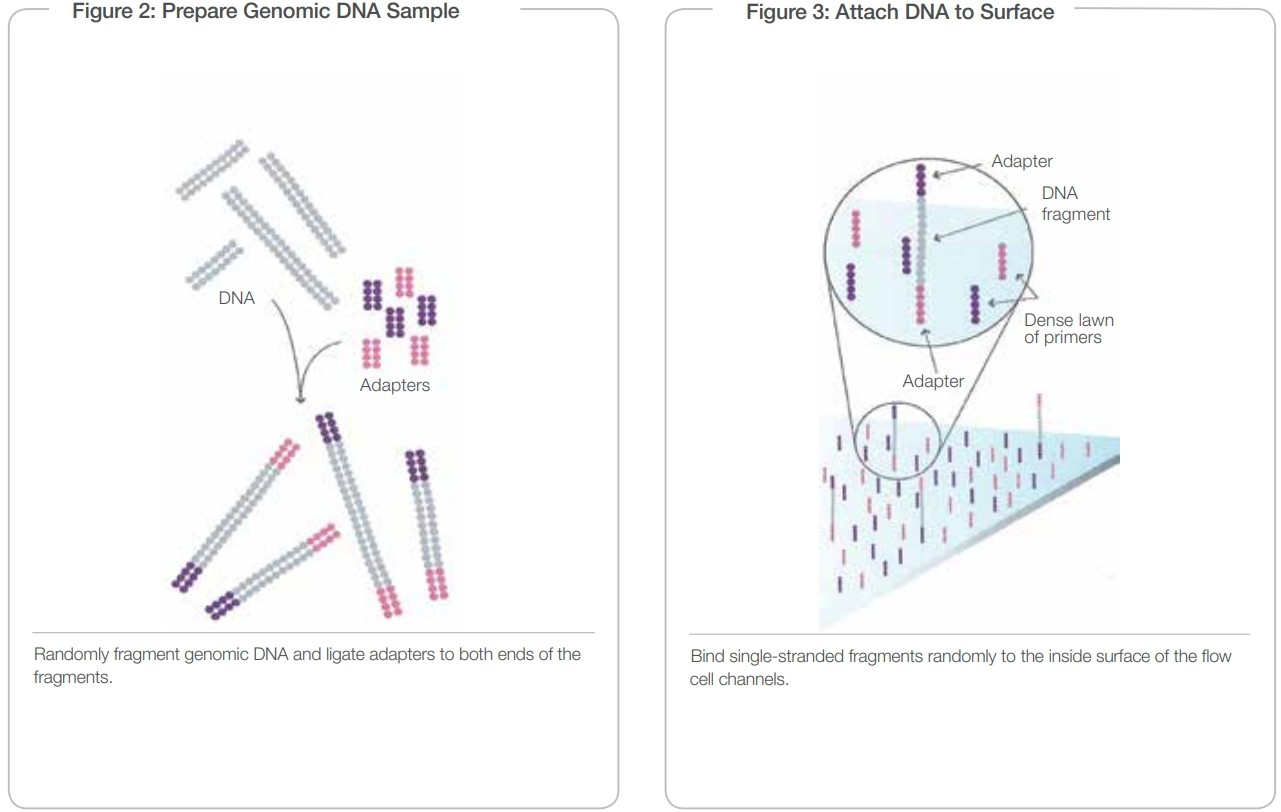
\includegraphics[scale=0.2]{illumina1.jpg}
\caption{Fragment DNA, ligate adaptor and oligos} 
\end{figure}
\end{frame}
% --- %
% -17- %
% --- %
\begin{frame}{Sequencing technology overview}
\framesubtitle{\emph{Illumina}}
\begin{figure}
\centering
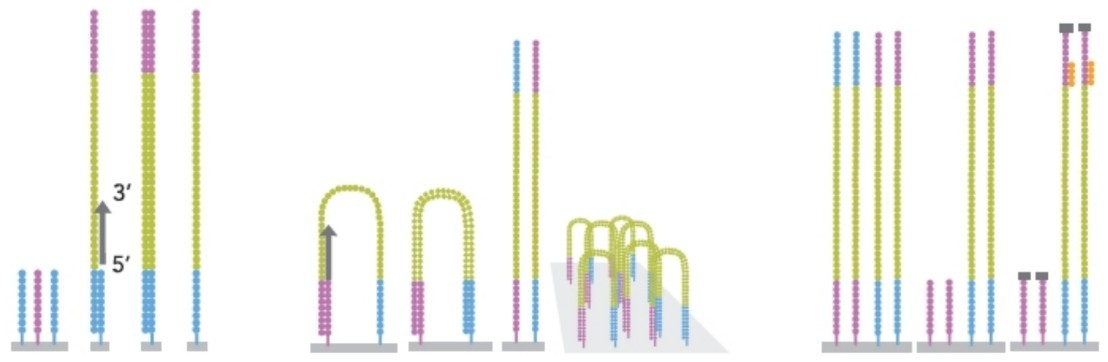
\includegraphics[scale=0.25]{illumina_extra.jpg}
\caption{Surface-bound primers are extended by DNA polymerase across annealed ssDNA molecules, the DNA is denatured back to single strands, and the free ends of immobilized strands anneal again to oligos bound on surface of flowcell. This ‘bridge PCR’ continues until a cluster of approximately 1000 molecules is produced on the surface of the flowcell, all descended from the single molecule that bound at that site. After PCR, the free ends of all DNA strands are blocked.} 
\end{figure}
\end{frame}
% --- %
% -18- %
% --- %
\begin{frame}{Sequencing technology overview}
\framesubtitle{\emph{Illumina}}
\begin{figure}
\centering
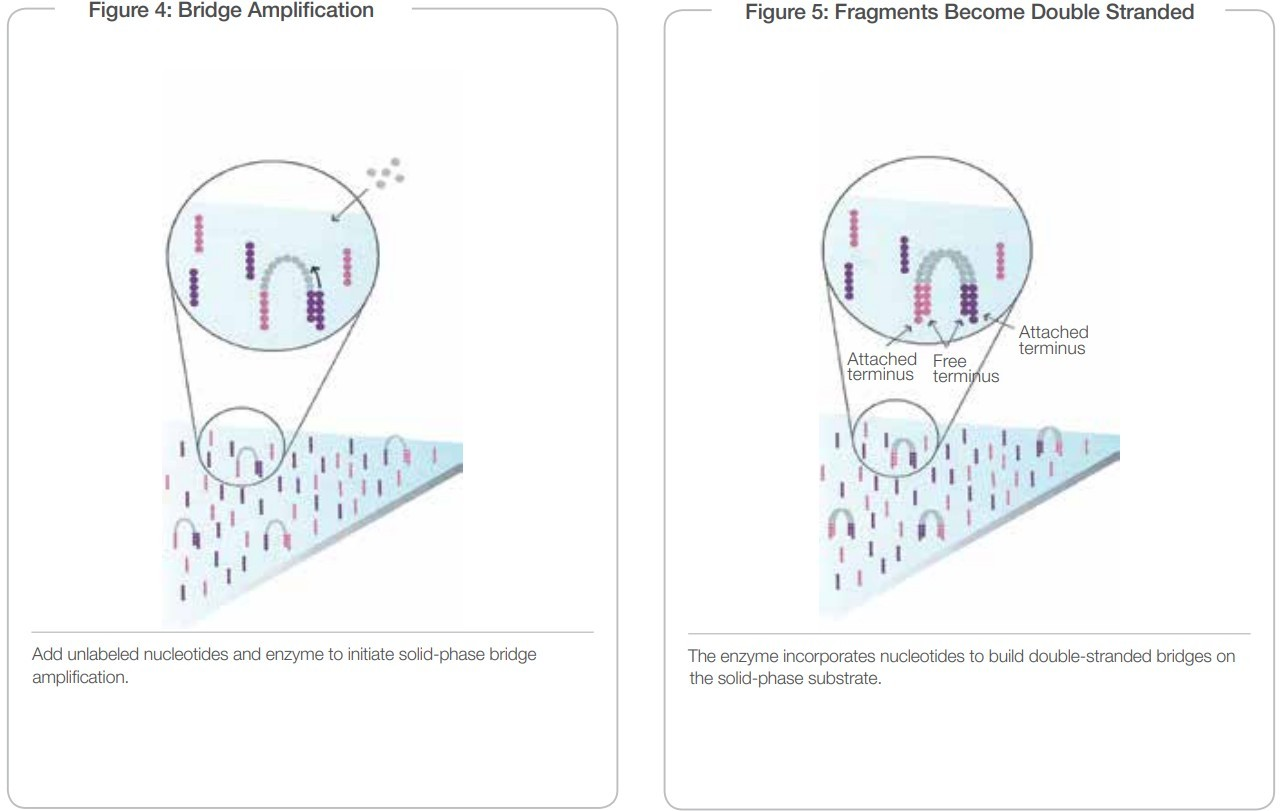
\includegraphics[scale=0.2]{illumina2.jpg}
\caption{Denaturalization and clusters of products} 
\end{figure}
\end{frame}
% --- %
% -19- %
% --- %
\begin{frame}{Sequencing technology overview}
\framesubtitle{\emph{Illumina}}
\begin{figure}
\centering
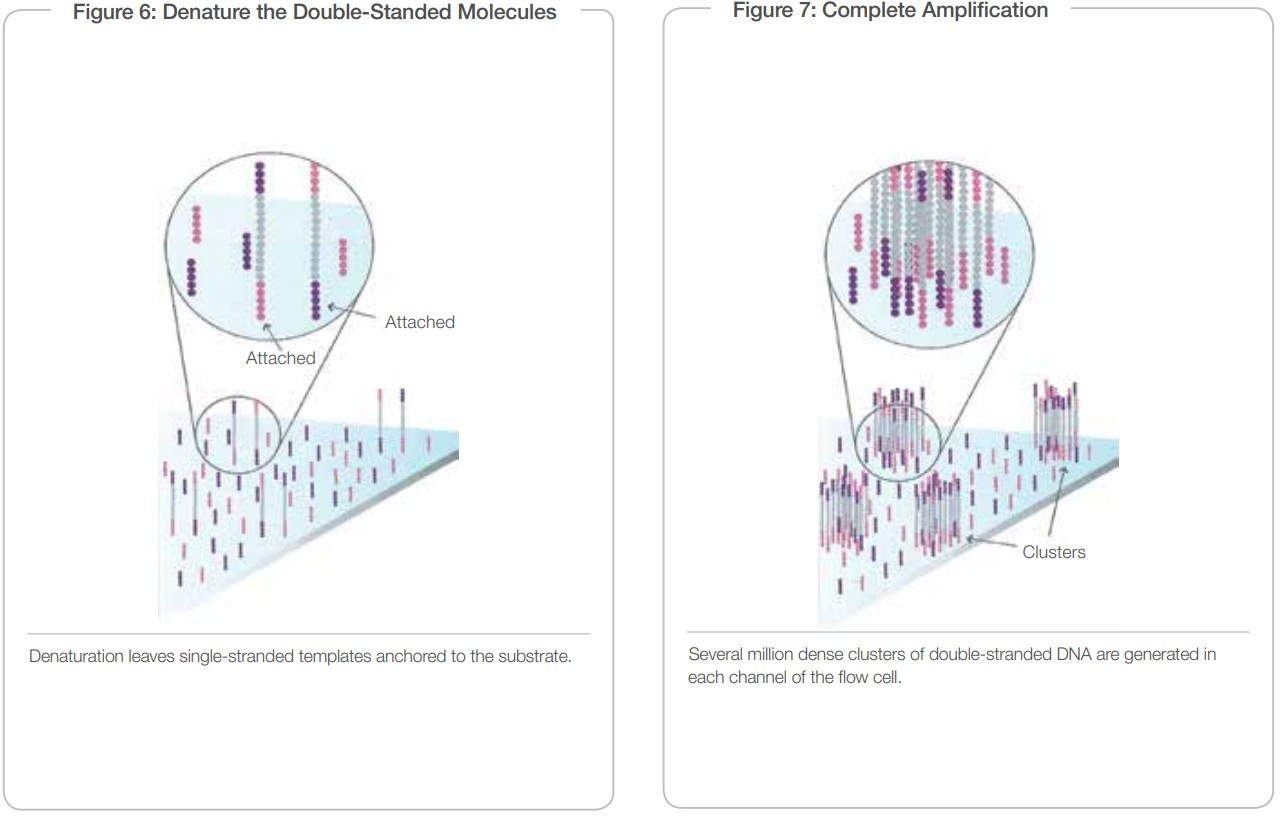
\includegraphics[scale=0.2]{illumina3.jpg}
\end{figure}
\end{frame}
% --- %
% -20- %
% --- %
\begin{frame}{Sequencing technology overview}
\framesubtitle{\emph{Illumina}}
\begin{figure}
\centering
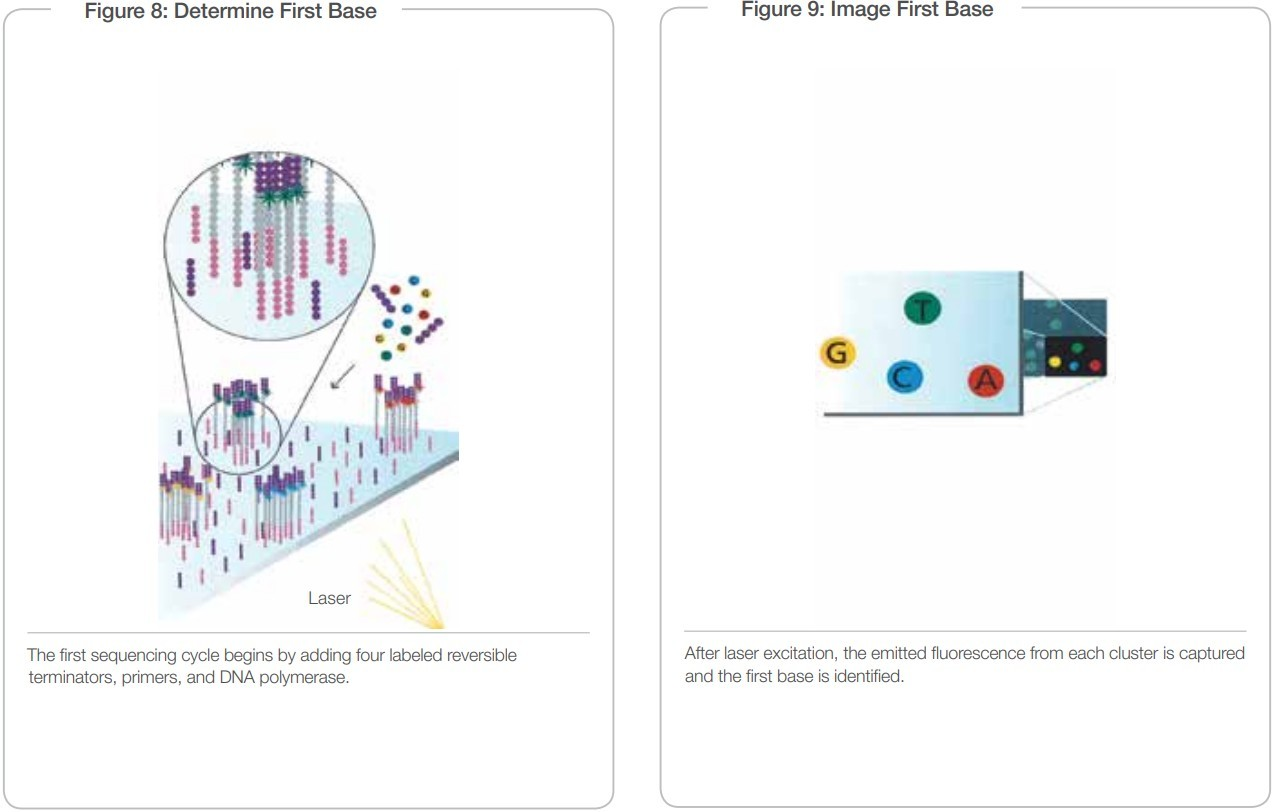
\includegraphics[scale=0.2]{illumina4.jpg}
\end{figure}
\end{frame}
% --- %
% -21- %
% --- %
\begin{frame}{Sequencing technology overview}
\framesubtitle{\emph{Illumina}}
\begin{figure}
\centering
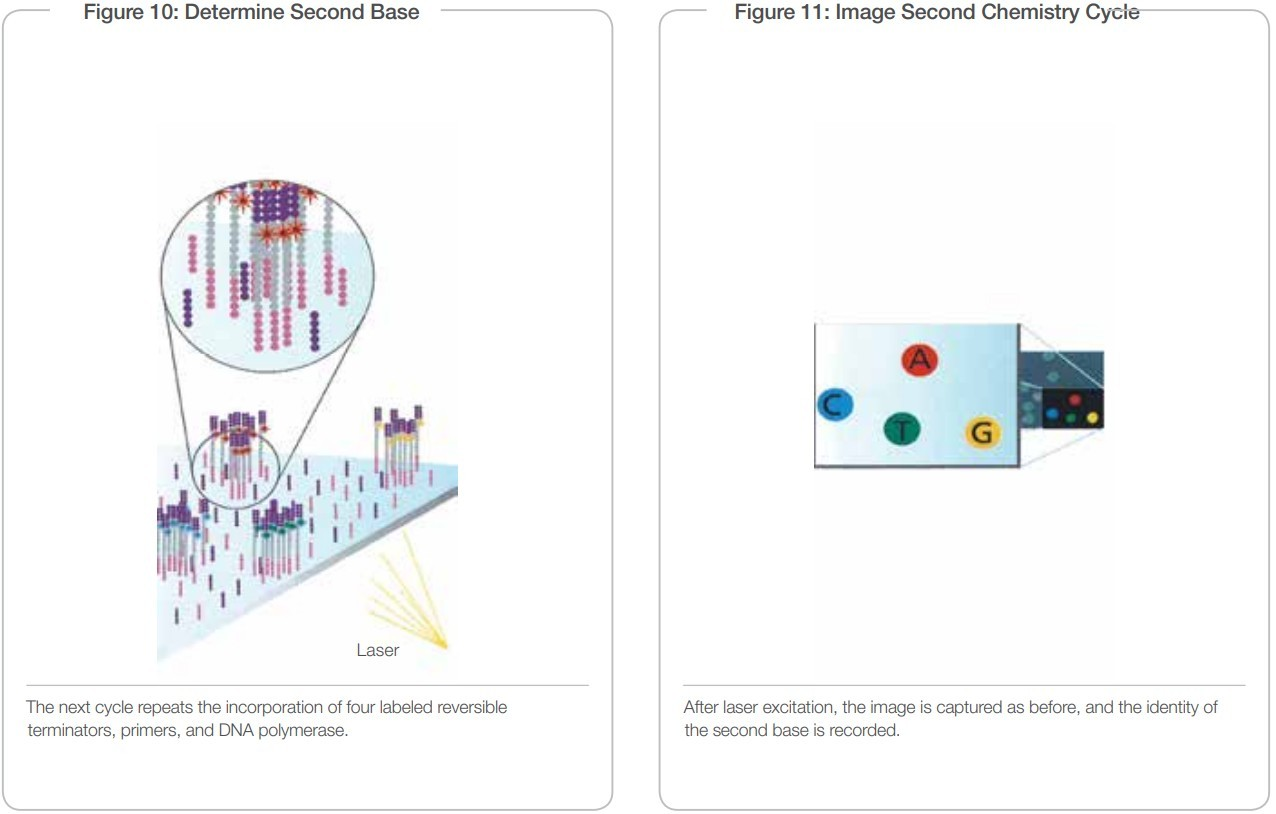
\includegraphics[scale=0.2]{illumina5.jpg}
\end{figure}
\end{frame}
% --- %
% -22- %
% --- %
\begin{frame}{Sequencing technology overview}
\framesubtitle{\emph{Illumina}}
\begin{figure}
\centering
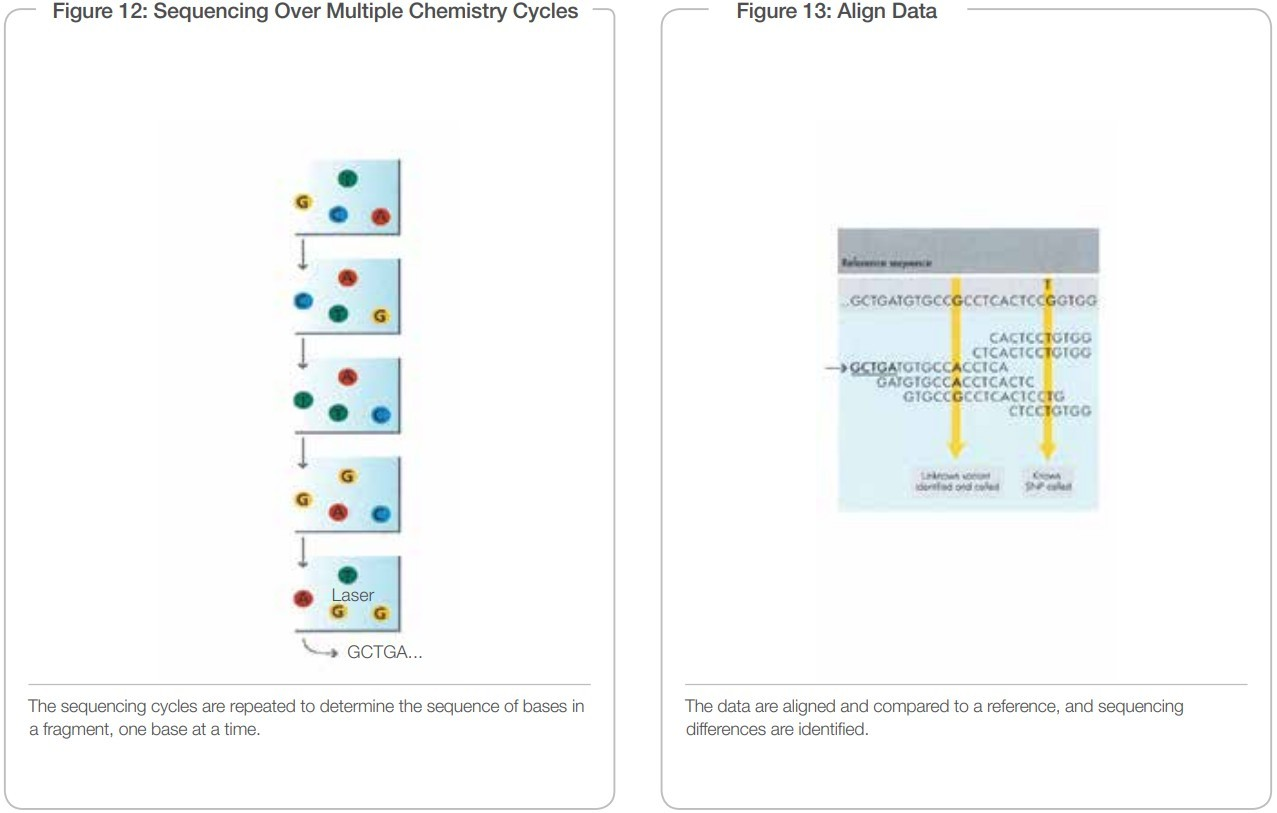
\includegraphics[scale=0.2]{illumina6.jpg}
\end{figure}
\end{frame}

\section{NGS File Formats}
% --- %
% -1- %
% --- %
\begin{frame}{NGS Bioinformatics Pipeline}
\begin{large}
\begin{itemize}
    \item Quality Control of FASTQ sentence files.
    \item Read mapping against some Reference Genome.
    \item Analysis of the mapped reads:
    \begin{itemize}
        \item Variant Calling (Exome, genome...)
        \item Differential Expression (RNA-seq)
        \item Peak calling (ChIP-seq)
    \end{itemize}
    \item Visualization.
    \item Biomedical interpretation.
\end{itemize} 
\end{large}
\end{frame}
% --- %
% -2- %
% --- %
\begin{frame}{NGS Bioinformatics Pipeline}
\begin{figure}
\centering
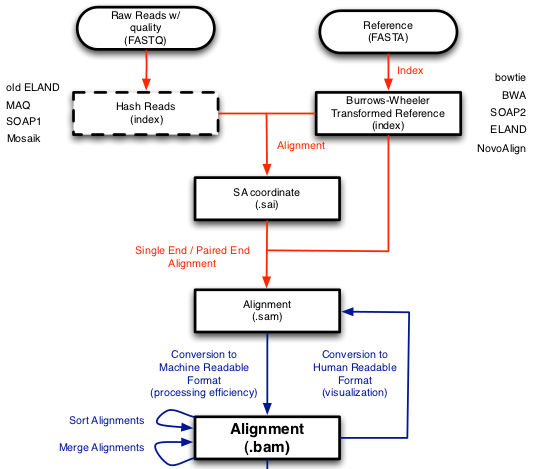
\includegraphics[scale=0.6]{ngs_scheme.png}
\end{figure}
\end{frame}
% --- %
% -3- %
% --- %
\begin{frame}{NGS File Formats}
\begin{large}
\begin{itemize}
    \item Many different file formats that reflect the various steps of analysis.
    \item We are going to introduce the most common formats today.
    \item Some of them are going to be used in our Hands-On 
    \item Remaining lectures will fill in details and lead into another types of analysis with another formats.
\end{itemize} 
\end{large}
\end{frame}
% --- %
% -4- %
% --- %
\begin{frame}{NGS File Formats}
\framesubtitle{\emph{Sequence data output format}}
\begin{itemize}
    \item DNA sequence data are typically provided with \textit{quality scores}, either as paired files or combined in a FASTQ file.
    \item In separate files, DNA sequences are in \cref{https://en.wikipedia.org/wiki/FASTA_format}{FASTA format}
    \begin{figure}
    \centering
    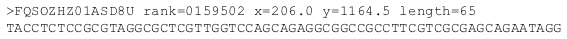
\includegraphics[scale=0.6]{fasta_sample.PNG}
    \end{figure}
    \item and quality scores are numbers from 0 to 40 (SCARF format)
    \begin{figure}
    \centering
    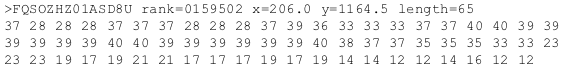
\includegraphics[scale=0.6]{scarf_sample.PNG}
    \end{figure}
    \item In \cref{https://en.wikipedia.org/wiki/FASTQ_format}{FASTQ format} , DNA sequences look similar, but quality scores are encoded as single text characters rather than as numbers
    \begin{figure}
    \centering
    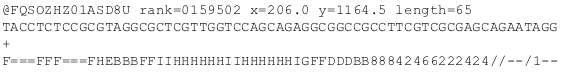
\includegraphics[scale=0.6]{fastq_sample.PNG}
    \end{figure}
\end{itemize} 
\end{frame}
% --- %
% -5- %
% --- %
\begin{frame}{NGS File Formats}
\framesubtitle{\emph{Understanding FASTQ format}}
\begin{itemize}
    \item Most recent Illumina Sequences are reported in FASTQ format
    \begin{figure}
    \centering
    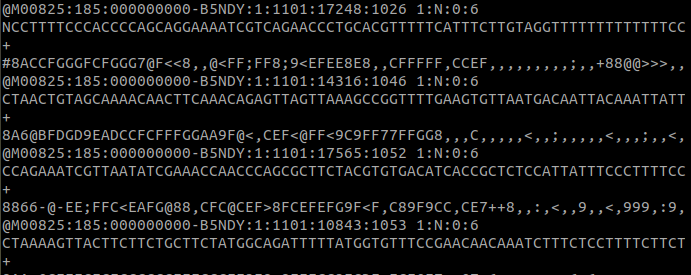
\includegraphics[scale=0.5]{fastq.PNG}
    \end{figure}
    \begin{enumerate}
        \item Read identifier
        \begin{itemize}
            \item Unique instrument name
            \item Run id
            \item Flowcell id
            \item Flowcell lane
            \item Number within the flowcell lane
            \item x-coordinate of the cluster within the tile
            \item y-coordinate of the cluster within the tile
            \item the member of a pair, 1 or 2 (paired-end or mate-pair reads only)
            \item Y if the read is filtered, N otherwise
            \item 0 when none of the control bits are on, otherwise it is an even number
            \item sample number
        \end{itemize}
    \end{enumerate}
\end{itemize} 
\end{frame}
% --- %
% -6- %
% --- %
\begin{frame}{NGS File Formats}
\framesubtitle{\emph{Understanding FASTQ format}}
\begin{itemize}
    \item Most recent Illumina Sequences are reported in FASTQ format
    \begin{enumerate}
        \item Read identifier
        \item Raw sequence reported by the machine
        \item '+' (can optionally include a sequence description)
        \item The FASTQ format encodes \cref{https://en.wikipedia.org/wiki/Phred_quality_score}{PHRED scores} as ASCII characters alongside the read sequences.
    \end{enumerate}
    \item Quality scores are numbers which represent the probability that the given base call is an error.
    \item These probabilities are always less than 1, so the value is given as -10x(log10) of the probability.
    \item An error probability of 0.001 is represented as a quality of score of 30.
    \item The numbers are converted into text characters so they occupy less space. A single character is as meaningful as 2 numbers plus a space between adjacent values. 
\end{itemize} 
\end{frame}
% --- %
% -7- %
% --- %
\begin{frame}{NGS File Formats}
\framesubtitle{\emph{Understanding FASTQ format}}
\begin{itemize}
    \item Unfortunately, at least 4 different ways of \textbf{converting numbers} to characters have been widely used, and \textbf{header line formats} have also changed, so one aspect of data analysis is knowing what you have.
\end{itemize} 
\begin{figure}
\centering
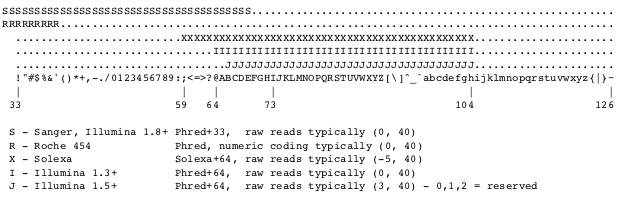
\includegraphics[scale=0.7]{ref_table_quality1.PNG}
\caption{Reference table}
\end{figure}
\end{frame}
% --- %
% -8- %
% --- %
\begin{frame}{NGS File Formats}
\framesubtitle{\emph{Understanding FASTQ format}}
\begin{itemize}
    \item Unfortunately, at least 4 different ways of \textbf{converting numbers} to characters have been widely used, and \textbf{header line formats} have also changed, so one aspect of data analysis is knowing what you have.
\end{itemize} 
\begin{figure}
\centering
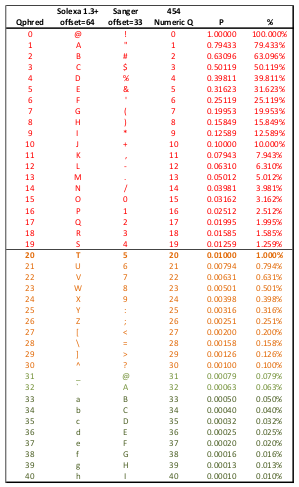
\includegraphics[scale=0.4]{ref_table_quality2.PNG}
\caption{Reference table}
\end{figure}
\end{frame}
% --- %
% -9- %
% --- %
\begin{frame}{NGS File Formats}
\framesubtitle{\emph{Understanding FASTQ format}}
\begin{figure}
\centering
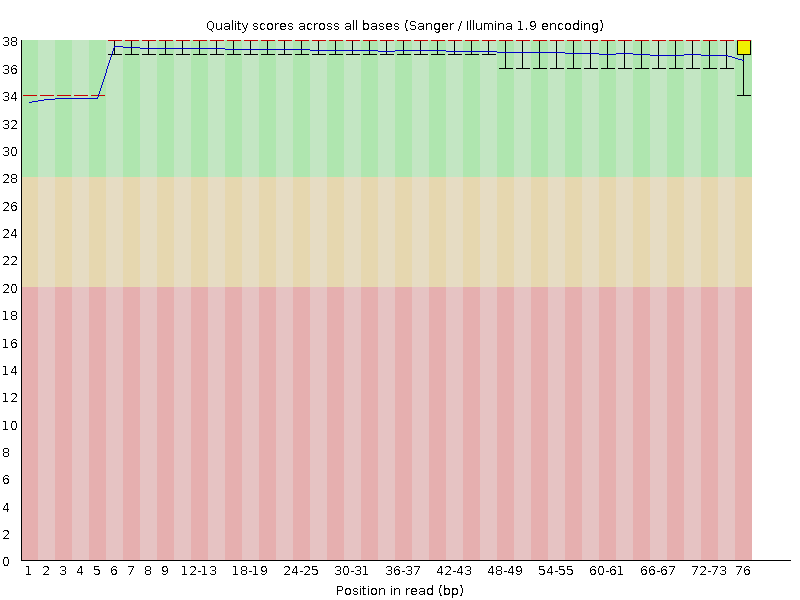
\includegraphics[scale=0.3]{per_base_quality.png}
\caption{Practical per base quality view generated with FastQC package}
\end{figure}
\end{frame}

\section{Read Mapping and Alignments}
% --- %
% -1- %
% --- %
\begin{frame}{NGS Bioinformatics Pipeline}
\begin{figure}
\centering
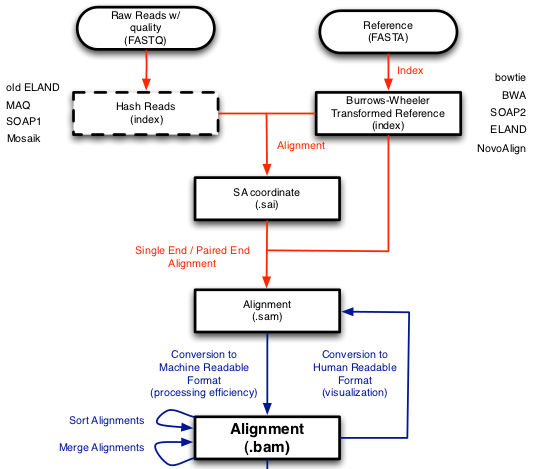
\includegraphics[scale=0.6]{ngs_scheme.png}
\end{figure}
\end{frame}
% --- %
% -2- %
% --- %
\begin{frame}{Read Mapping and Alignments}
Once high-quality data are obtained from preprocessing, the next step is the read mapping or alignment. 
\\~\\
There are two main options depending on the availability of a genome sequence
\begin{itemize}
    \item When studying an organism with a \textbf{reference genome}, it is possible to infer which transcripts are expressed by mapping the reads to the reference genome (\textbf{genome mapping}) or transcriptome (\textbf{transcriptome mapping}). Mapping reads to the genome requires no knowledge of the set of transcribed regions or the way in which exons are spliced together. This approach allows the discovery of new, unannotated transcripts.
    \item When working on an organism without a reference genome, reads need to be assembled first into longer contigs (\textbf{\textit{de novo assembly}}). These contigs can then be considered as the expressed transcriptome to which reads are re-mapped for quantification. \textit{De novo assembly} algorithms are constructed with de Bruijn graphs.
\end{itemize} 
\end{frame}
% --- %
% -3- %
% --- %
\begin{frame}{Read Mapping and Alignments}
\begin{figure}
\centering
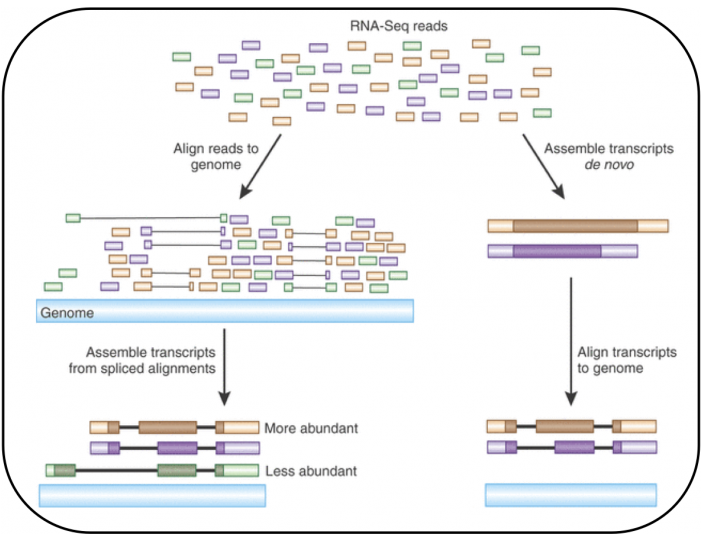
\includegraphics[scale=0.4]{rna_seq_align.PNG}
\caption{Mapping reads to a reference or de novo assembly}
\end{figure}
\end{frame}
% --- %
% -4- %
% --- %
\begin{frame}{Read Mapping and Alignments}
\begin{figure}
\centering
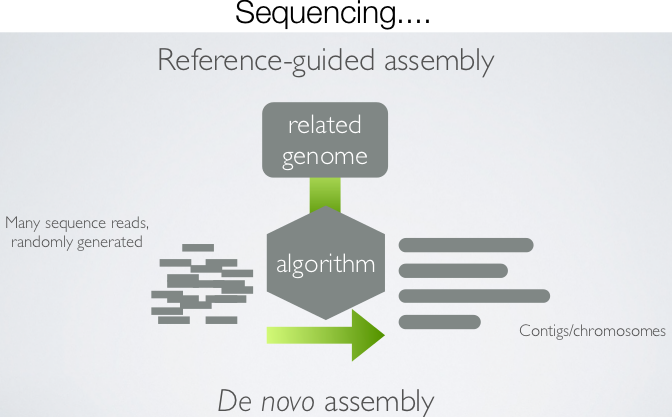
\includegraphics[scale=0.5]{sequencing.PNG}
\end{figure}
\end{frame}
% --- %
% -5- %
% --- %
\begin{frame}{Read Mapping and Alignments}
\begin{figure}
\centering
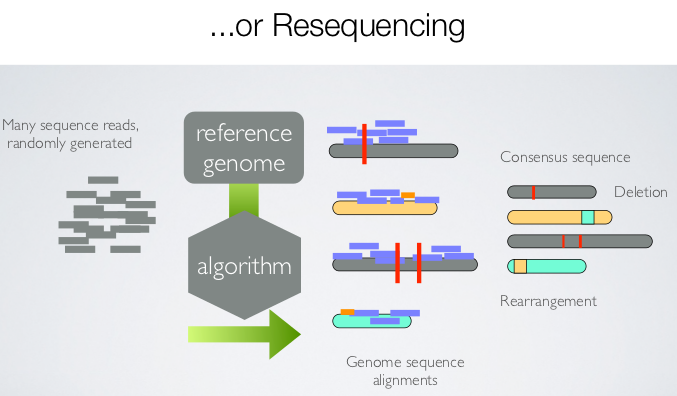
\includegraphics[scale=0.5]{resequencing.PNG}
\end{figure}
\end{frame}
% --- %
% -6- %
% --- %
\begin{frame}{Read Mapping and Alignments}
\framesubtitle{\emph{How to map billions of short reads onto genomes}}
\begin{figure}
\centering
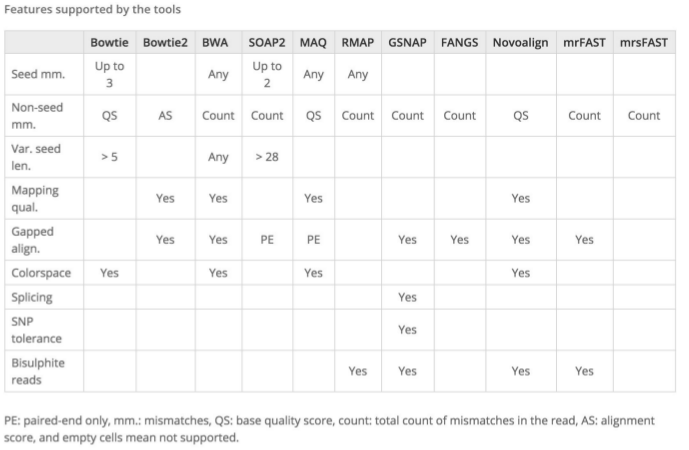
\includegraphics[scale=0.475]{aligners_comparison.PNG}
\end{figure}
\end{frame}
% --- %
% -7- %
% --- %
\begin{frame}{Reference Based Assembly}
\framesubtitle{\emph{The Burrows–Wheeler transform}}
\begin{figure}
\centering
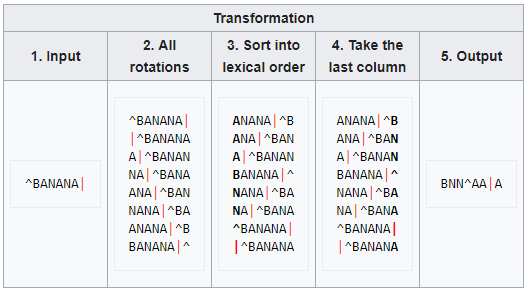
\includegraphics[scale=0.475]{bwt_banana.PNG}
\caption{The \cref{https://en.wikipedia.org/wiki/Burrows-Wheeler_transform}{\textbf{Burrows–Wheeler transform}} (BWT, also called block-sorting compression) rearranges a character string into runs of similar characters. This is useful for compression, since it tends to be easy to compress a string that has runs of repeated characters by techniques such as move-to-front transform and run-length encoding. More importantly, the transformation is \textbf{reversible}, without needing to store any additional data except the position of the first original character. The BWT is thus a "free" method of improving the efficiency of text compression algorithms, costing only some extra computation.}
\end{figure}
\end{frame}
% --- %
% -8- %
% --- %
\begin{frame}{Reference Based Assembly}
\framesubtitle{\emph{The Burrows–Wheeler transform}}
\begin{large}
\begin{itemize}
    \item When a string of characters is transformed by the BWT, none of its characters change the value (it is a \textbf{lossless compression algorithm}).
    \item The transformation changes the order of the characters. If the original string had several \textbf{substrings} that occurred frequently, then the transformed string has several sites where a single character is repeated consecutively.
    \item  This is very useful in \textbf{compression}: it is easier to compress a string that has several characters repeated together with techniques such as RLE encoding (run-length encoding).
\end{itemize} 
\end{large}
\end{frame}
% --- %
% -9- %
% --- %
\begin{frame}{Reference Based Assembly}
\framesubtitle{\emph{The Burrows–Wheeler transform}}
\begin{figure}
\centering
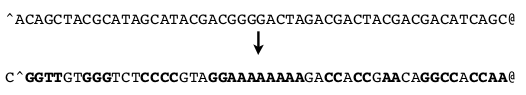
\includegraphics[scale=0.6]{example_bwt_sequence1.PNG}
\end{figure}
\begin{figure}
\centering
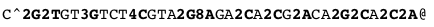
\includegraphics[scale=0.6]{example_bwt_sequence2.PNG}
\caption{BWT example with DNA. From 54 to 45 characters with this transformation}
\end{figure}
\end{frame}
% --- %
% -10- %
% --- %
\begin{frame}{Reference Based Assembly}
\begin{figure}
\centering
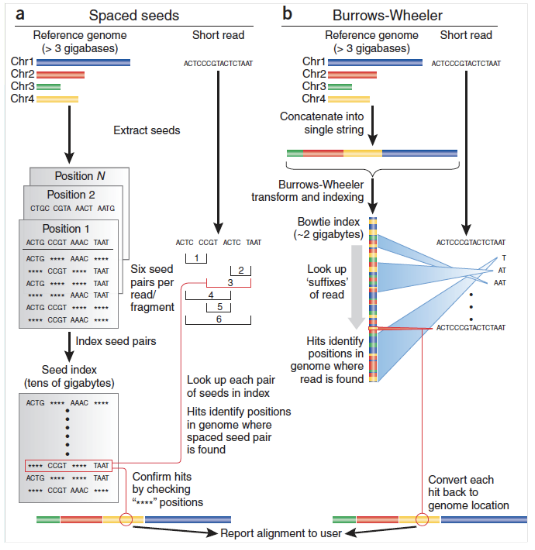
\includegraphics[scale=0.5]{bwt.PNG}
\end{figure}
\end{frame}
% --- %
% -11- %
% --- %
\begin{frame}{NGS File Formats}
\framesubtitle{\emph{SAM (Sequence Alignment/Map) format}}
\begin{itemize}
    \item \cref{https://en.wikipedia.org/wiki/SAM_(file_format)}{\textbf{SAM (Sequence Alignment/Map)}} is a generic format for storing large nucleotide sequence
    alignments.
    \item SAM is is the human readable, scriptable format. A \cref{https://support.illumina.com/help/BS_App_MDProcessor_Online_1000000007932/Content/Source/Informatics/BAM-Format.htm}{\textbf{BAM}} file is essentially a binary (gzip-compressed) version of a SAM file.
    \item  SAM/BAM files are usually sorted and indexed to streamline data
    processing. Both contains exactly the same information, and are interconvertible
\end{itemize} 
\begin{figure}
\centering
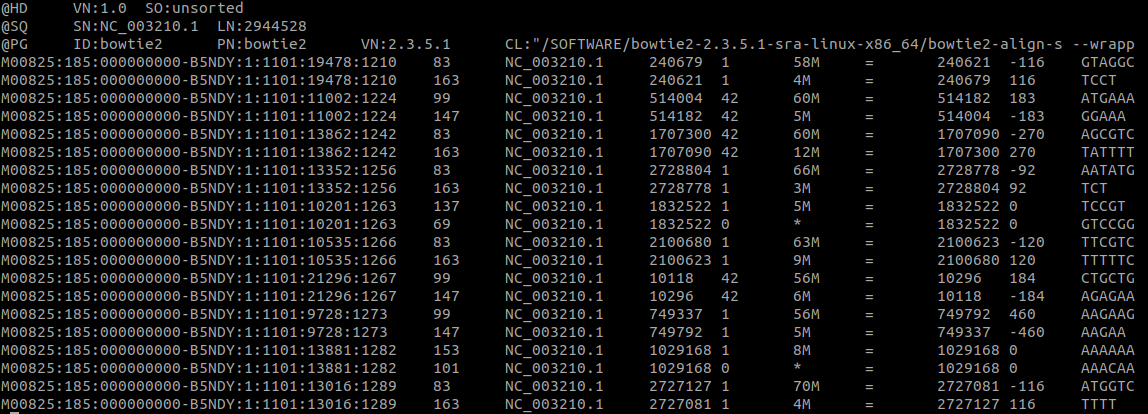
\includegraphics[scale=0.3]{sam_listeria.PNG}
\caption{SAM file format sample file}
\end{figure}
\end{frame}
% --- %
% -12- %
% --- %
\begin{frame}{NGS File Formats}
\framesubtitle{\emph{SAM (Sequence Alignment/Map) format}}
\begin{figure}
\centering
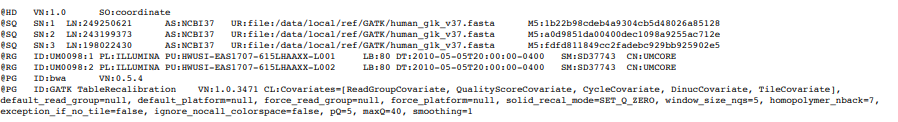
\includegraphics[scale=0.5]{sam_header.PNG}
\caption{SAM file format Header}
\end{figure}
\begin{figure}
\centering
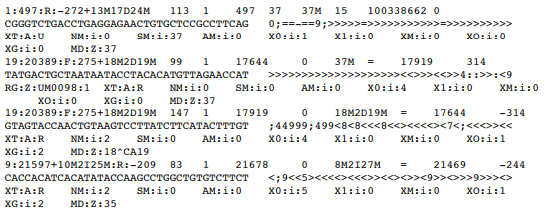
\includegraphics[scale=0.6]{sam_alignment.PNG}
\caption{SAM file format Alignment}
\end{figure}
\end{frame}
% --- %
% -13- %
% --- %
\begin{frame}{NGS File Formats}
\framesubtitle{\emph{SAM (Sequence Alignment/Map) format}}
\begin{figure}
\centering
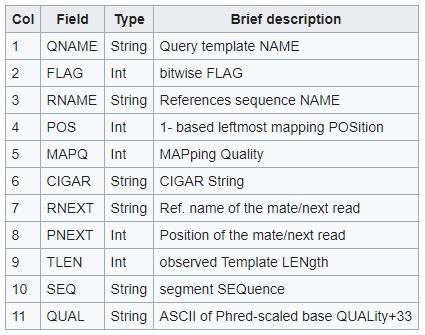
\includegraphics[scale=0.65]{sam_alignment_meaning.PNG}
\caption{Alignment sections have 11 mandatory fields}
\end{figure}
\end{frame}
% --- %
% -14- %
% --- %
\begin{frame}{NGS File Formats}
\framesubtitle{\emph{SAM (Sequence Alignment/Map) format}}
\begin{huge}
\centering
What is a CIGAR?
\\~\\
\end{huge}
The \cref{https://jef.works/blog/2017/03/28/CIGAR-strings-for-dummies/}{CIGAR} (Compact Idiosyncratic Gapped Alignment Report) string is how the SAM/BAM format represents spliced alignments. Understanding the CIGAR string will help you \textbf{understand how your query sequence aligns to the reference genome}.
\begin{figure}
\centering
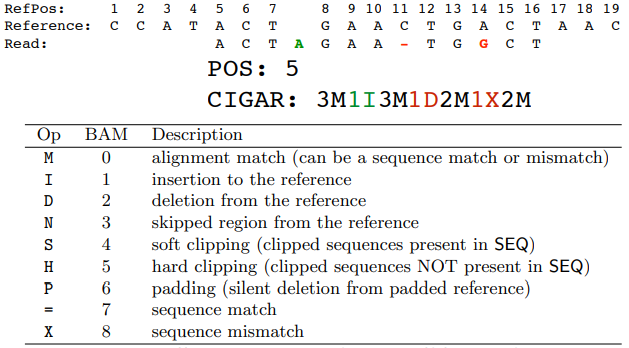
\includegraphics[scale=0.5]{cigar.PNG}
\end{figure}
\end{frame}
% --- %
% -15- %
% --- %
\begin{frame}{NGS File Formats}
\framesubtitle{\emph{Other interesting NGS data format files}}
\begin{huge}
\centering
Annotation files
\\~\\
\end{huge}
\centering
\cref{https://en.wikipedia.org/wiki/General_feature_format}{GFF (General Feature Format)}, \cref{https://en.wikipedia.org/wiki/Gene_transfer_format}{GTF (Gene Transfer format)}, \cref{https://www.ensembl.org/info/website/upload/gff3.html}{GFF3} or \cref{https://www.ensembl.org/info/website/upload/bed.html}{BED (Browser Extensible Data)}
\begin{figure}
\centering
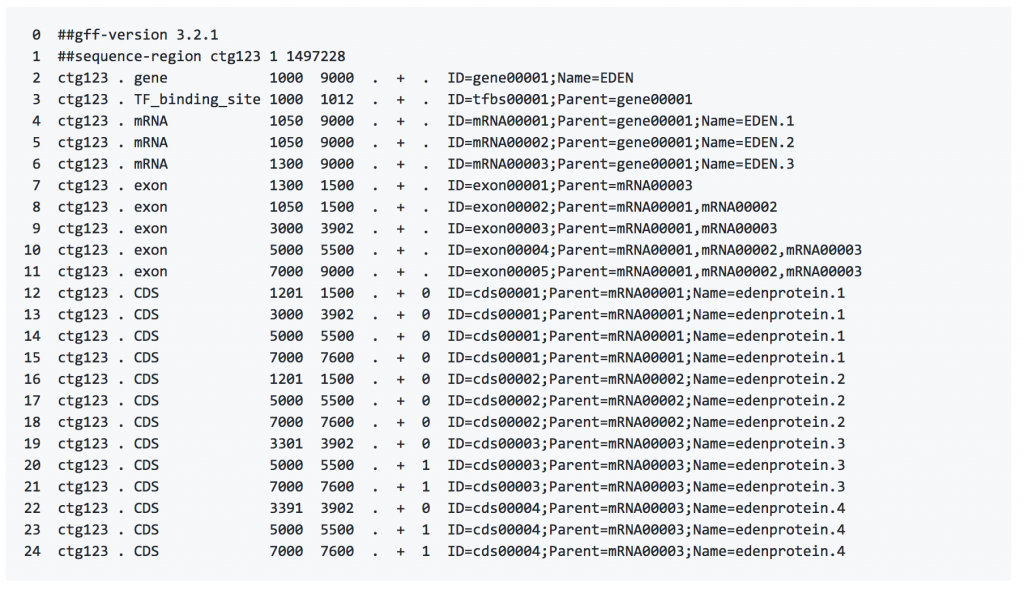
\includegraphics[scale=0.2]{gff3.png}
\caption{GFF3 sample file}
\end{figure}
\end{frame}
% --- %
% -16- %
% --- %
\begin{frame}{NGS File Formats}
\framesubtitle{\emph{Other interesting NGS data format files}}
\begin{huge}
\centering
The Variant Call Format
\\~\\
\end{huge}
\centering
\cref{https://samtools.github.io/hts-specs/VCFv4.2.pdf}{VCF}
\begin{figure}
\centering
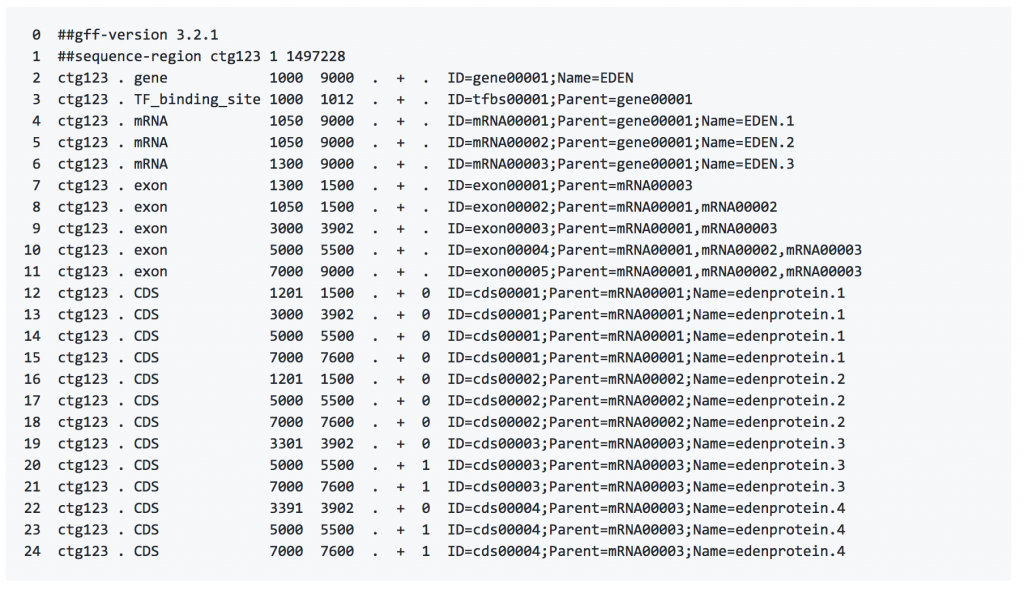
\includegraphics[scale=0.2]{gff3.png}
\caption{Variant Call Format (VCF) sample file}
\end{figure}
\end{frame}
% --- %
% -1- %
% --- %
\section{Linux Command-Line Interface}
\begin{frame}{Why we need an Operating System (OS)?}
\begin{figure}
\centering
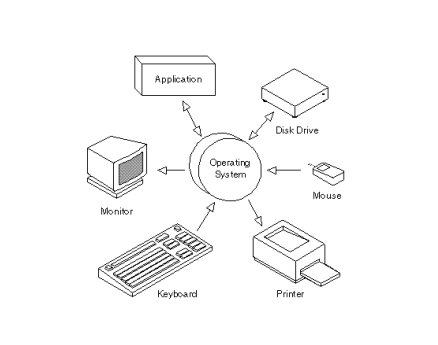
\includegraphics[scale=0.6]{operating_system_components.PNG}
\caption{An operating system (OS) is system software that manages computer hardware and software resources and provides common services for computer programs}
\end{figure}
\end{frame}
% --- %
% -5- %
% --- %
\begin{frame}{Why we need an Operating System (OS)?}
\begin{figure}
\centering
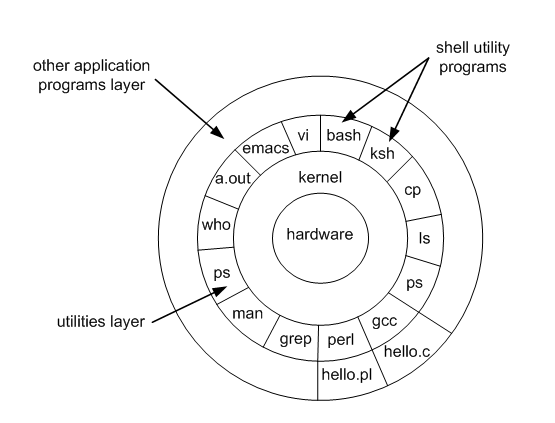
\includegraphics[scale=0.55]{linux_layers.PNG}
\caption{Linux Layers}
\end{figure}
\end{frame}
% --- %
% -2- %
% --- %
\begin{frame}{Linux Distributions}
\begin{figure}
\centering
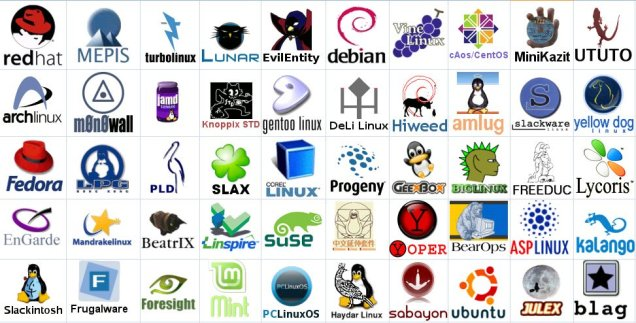
\includegraphics[scale=0.5]{linux_distros.jpg}
\caption{Ubuntu will be our OS to manage the Hands-on session}
\end{figure}
\end{frame}
% --- %
% -3- %
% --- %
\begin{frame}{Why use Linux for sequencing data?}
\begin{figure}
\centering
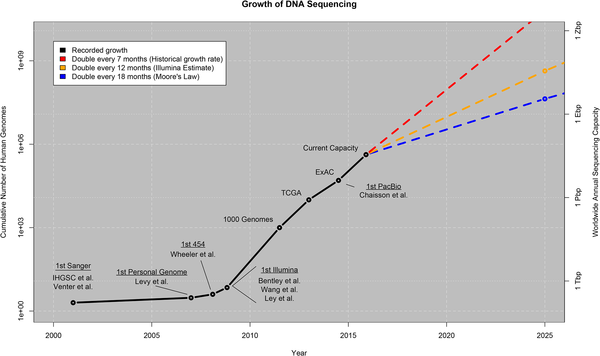
\includegraphics[scale=2]{linux_plois.PNG}
\caption{Growth of DNA Sequencing (Stephens et al. PLoS Biol. 2015)}
\end{figure}
\end{frame}
% --- %
% -4- %
% --- %
\begin{frame}{Why use Linux for sequencing data?}
\begin{large}
\begin{itemize}
    \item Thousand of tools that each do simple tasks.
    \item Preferred development platform for \textbf{open-source} software.
    \item Free.
    \item Built for \textbf{speed}, not for ...
\end{itemize}
Some alternatives exist:
\begin{itemize}
    \item Java / C++ programs. Run on any major operating system.
    \item Mac OS X is Linux based OS with a very nice GUI.
    \item Commercial software exist.
\end{itemize}
\end{large}
\end{frame}
% --- %
% -5- %
% --- %
\begin{frame}{Linux Directory Structure}
\begin{figure}
\centering
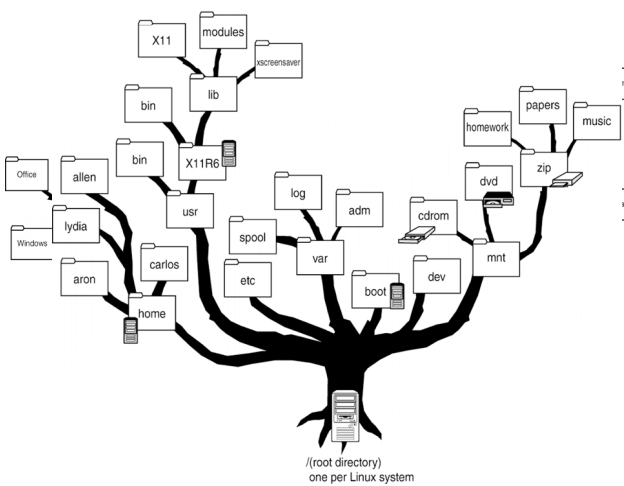
\includegraphics[scale=0.5]{linux_directories.PNG}
\end{figure}
\end{frame}
% --- %
% -5- %
% --- %
\begin{frame}{Sample Linux Paths}
\begin{figure}
\centering
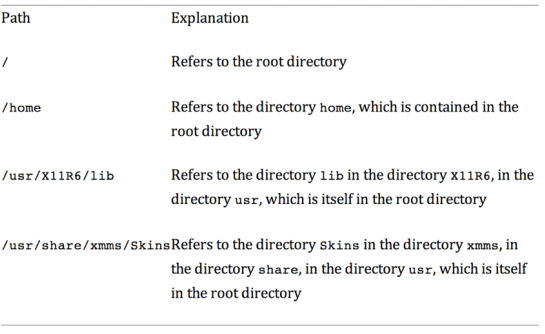
\includegraphics[scale=0.6]{linux_paths.PNG}
\end{figure}
\end{frame}
% --- %
% -5- %
% --- %
\begin{frame}{Linux Commands}
\begin{alertblock}{Basic Commands}
\begin{enumerate}
    \item \textbf{pwd} - When you first open the terminal, you are in the home directory of your user.
    \item \textbf{ls} - Use this command to know what files are in the directory you are in. You can see all the hidden files by using the command \textbf{ls -a}.
    \item \textbf{cd} - Use the "cd" command to go to a directory.
    \item \textbf{mkdir \& rmdir} - Use the mkdir command when you need to create a folder or a directory. Use rmdir to delete a directory.
    \item \textbf{rm} - Use the rm command to delete files and directories.  Use \textbf{rm -r} to delete just the directory. It deletes both the folder and the files it contains when using only the rm command.
    \item \textbf{touch} -  The touch command is used to create a file.
    \item \textbf{man \& --help} - To know more about a command and how to use it, use the man command.
    \item \textbf{cp} - Use the cp command to copy files through the command line.
    \item \textbf{mv } -  Use the mv command to move files through the command line.
    \item \textbf{locate } - The locate command is used to locate a file in a Linux system, just like the search command in Windows. 
\end{enumerate}
\end{alertblock}
\end{frame}
% --- %
% -6- %
% --- %
\begin{frame}{Linux Commands}
\begin{alertblock}{Intermediate Commands}
\begin{enumerate}
    \item \textbf{echo} - If you want to create a new text file or add to an already made text file, you just need to type in \textbf{echo hello, my name is alok >> new.txt}.
    \item \textbf{cat} - Use the cat command to display the contents of a file. It is usually used to easily view programs.
    \item \textbf{nano, vi, jed} - nano and vi are already installed text editors in the Linux command line. 
    \item \textbf{sudo} - If you want any command to be done with administrative or root privileges, you can use the sudo command.
    \item \textbf{df} - Use the df command to see the available disk space in each of the partitions in your system. 
    \item \textbf{du} - Use du to know the disk usage of a file in your system. 
    \item \textbf{tar} - Use tar to work with tarballs (or files compressed in a tarball archive) in the Linux command line.
    \item \textbf{zip, unzip} -  Use zip to compress files into a zip archive, and unzip to extract files from a zip archive.
    \item \textbf{uname} - Use uname to show the information about the system your Linux distro is running.
\end{enumerate}
\end{alertblock}
\end{frame}
% --- %
% -7- %
% --- %
\begin{frame}{Linux Commands}
\begin{large}
\centering
Tips and Tricks for Using Linux Command Line
\end{large}
\begin{itemize}
    \item You can use the \textbf{clear} command to clear the terminal if it gets filled up with too many commands.
    \item \textbf{TAB} can be used to fill up in terminal. For example, You just need to type \textbf{cd Doc} and then TAB and the terminal fills the rest up and makes it \textbf{cd Documents}.
    \item \textbf{Ctrl+C} can be used to stop any command in terminal safely. If it doesn't stop with that, then \textbf{Ctrl+Z} can be used to force stop it.
    \item You can exit from the terminal by using the \textbf{exit} command.
    \item You can power off or reboot the computer by using the command \textbf{reboot}.
    \item Use some \cref{https://files.fosswire.com/2007/08/fwunixref.pdf}{Unix Command Line References}
\end{itemize}
\end{frame}
% --- %
% -7- %
% --- %
\begin{frame}{Thank you for your attention !}
\centering
And now...
\begin{figure}
\centering
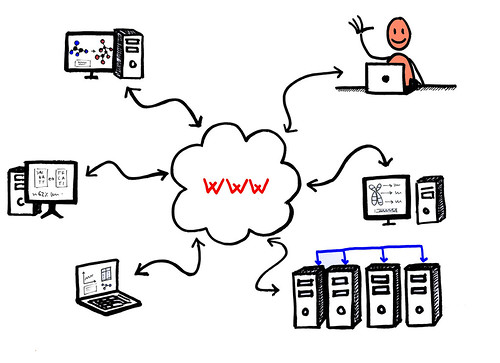
\includegraphics[scale=0.45]{hands-on.jpg}
\end{figure}
\end{frame}
% --- %
% -7- %
% --- %
\begin{frame}{Hands-on}
\centering
\begin{huge}
\exemple{Click on this \cref{https://github.com/fpozoc/advanced_bioinformatics}{link} to start the Hands-on:\\~\\ \textbf{Transcriptome Assembly: Case study of bacteria \textit{Listeria monocytogenes}}}
\end{huge}
\end{frame}
\end{document}
